\section{Task 2} \label{sec:Task2}

Nach der erfolgreichen Modellierung in PLECS wurde die Hardware-Implementierung vorbereitet. In diesem Kapitel werden die notwendigen Schritte zur Umsetzung erläutert. Dabei stehen die Echtzeitfähigkeit der RTBox, die Anbindung des Mikrocontrollers sowie die Entwicklung der Steueralgorithmen im Fokus. Die Herausforderungen der Echtzeitregelung und die erforderlichen Anpassungen werden ebenfalls behandelt. Abschließend erfolgt eine Analyse der Performance basierend auf Simulationen und experimentellen Ergebnissen.

Zur Umsetzung wurden zwei Subsysteme definiert – eines für den Controller, eines für das geregelte System. Diese Trennung ermöglicht eine separate Parametrierung der Coder-Optionen für eine optimierte Code-Generierung. Die Ein- und Ausgänge wurden wie folgt konfiguriert und miteinander verschaltet:

\begin{itemize}
    \item \textbf{System-Subsystem:} Enthält PLECS PWM Capture sowie PLECS Analog Out für Strom- und Spannungsmessung (Siehe Abbildung: Model_Task2_System.png)
 
    \item \textbf{Controller-Subsystem:} Enthält STM PWM Out für die Ansteuerung sowie STM ADC (Analog In Triggered) zur Erfassung der Systemrückmeldung. Ein Control Trigger Block wurde integriert, um den ADC korrekt zu triggern. (Siehe Abbildung: Model_Task2_Controller.png)
\end{itemize}

Die Simulation wurde mit zwei verschiedenen Lasten ($R_{Load}=\SI{2}{\ohm}$ und $R_{Load}=\SI{4}{\ohm}$) durchgeführt, um die Performance des Reglers unter verschiedenen Bedingungen zu bewerten. Das PLECS-Modell wurde schrittweise für die Hardware-Simulation mit der RTBox und dem STM32 Nucleo vorbereitet. Die in den Coder-Optionen gesetzten Parameter:

\begin{itemize}
    \item \textbf{Controller:} Target = STM32G4x; Scheduling Step Size = (Siehe Abbildung: Settings CoderOptions_Model_Task2_ControllerTarget.png)

    \item \textbf{System:} Target = PLECS RT Box 2; Scheduling Step Size =  (Siehe Abbildung: Settings CoderOptions_Model_Task2_SystemTarget.png)

    \item \textbf{Gesamtsystem-Ansicht:} Überblick der vollständigen Implementierung (Siehe Abbildung: Model_Task2.png)
\end{itemize}

\begin{figure}[H]
    \centering
    \includegraphics[width=0.6\linewidth]{Figure/Hard.png}
    \caption{FFT LTC3639 mit Filter}
    \label{fig:Hard}
\end{figure}

\begin{figure}[H]
    \centering
    \includegraphics[width=0.6\linewidth]{Figure/SystemHard.png}
    \caption{FFT LTC3639 mit Filter}
    \label{fig:SystemHard}
\end{figure}

\begin{figure}[H]
    \centering
    \includegraphics[width=0.6\linewidth]{Figure/ControllerHard.png}
    \caption{FFT LTC3639 mit Filter}
    \label{fig:ControllerHard}
\end{figure}





\subsection{Ergebnisse der Simulation an der Hardware}

Für die Evaluierung des Reglers wurden Simulationen mit zwei Lastwiderständen durchgeführt:

\begin{itemize}
    \item \textbf{Ergebnisse für $R_{Load}=\SI{2}{\ohm}$:} Die Simulation zeigt eine stabile Regelung mit geringer Überschwingung. Der Spannungsverlauf erreicht schnell den gewünschten Wert und bleibt stabil. (Siehe Abbildung: \ref{fig:Rload2})
    \item \textbf{Ergebnisse für $R_{Load}=\SI{4}{\ohm}$:} Auch bei einer höheren Last bleibt das System stabil. Die Regelung reagiert schnell und hält die Ausgangsspannung zuverlässig. Die Reaktionszeit ist etwas kürzer als bei $R_{Load}=\SI{2}{\ohm}$, was an der veränderten Systemdynamik liegt. (Siehe Abbildung: \ref{fig:Rload4})
\end{itemize}

\begin{figure}[H]
    \centering
    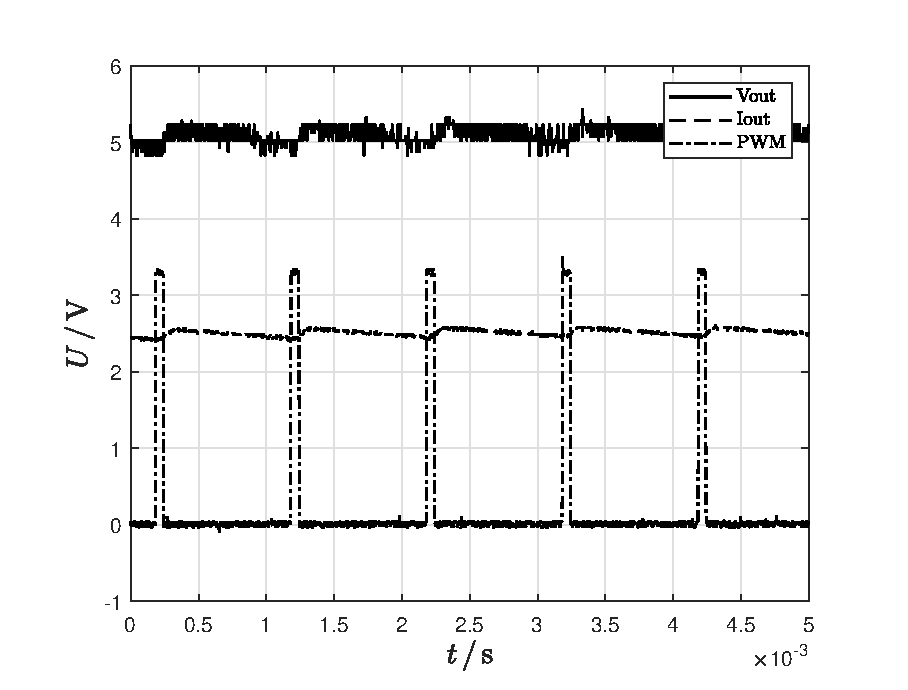
\includegraphics[width=0.6\linewidth]{Figure/Rload2.eps}
    \caption{Messung mit $R_{load} = \SI{2}{\ohm}$}
    \label{fig:Rload2}
\end{figure}

\begin{figure}[H]
    \centering
    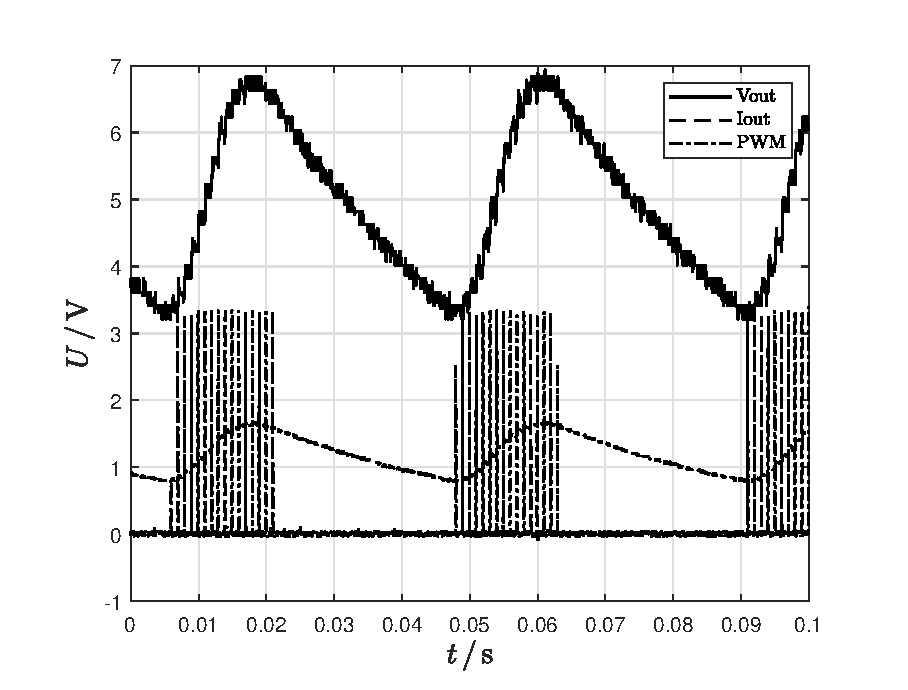
\includegraphics[width=0.6\linewidth]{Figure/Rload4.eps}
    \caption{Messung mit $R_{load} = \SI{4}{\ohm}$}
    \label{fig:Rload4}
\end{figure}